\documentclass[a4paper,12pt]{article}
\input{/Users/richard/Github/LaTex/preamble/preamble_article.tex}
\usepackage{titlesec}
\usepackage{fancyhdr}
\definecolor{navy}{RGB}{31,67,103}
\titleformat{\section}{\Large\bfseries\color{navy}}{\thesection}{0.7em}{}[\color{navy}\titlerule]
\titleformat{\subsection}{\large\bfseries\color{navy}}{\thesubsection}{0.6em}{}
\titleformat{\subsubsection}{\normalsize\bfseries\color{navy}}{\thesubsubsection}{0.6em}{}
\titlespacing*{\section}{0pt}{1.8ex plus .5ex}{1ex}
\setlist[itemize]{leftmargin=2.2em,itemsep=.45ex,topsep=.5ex,parsep=0pt}
\setlist[enumerate]{leftmargin=2.5em,itemsep=.8ex,topsep=.6ex}
\setlength{\headheight}{15pt}
\pagestyle{fancy}
\fancyhf{}
\fancyhead[L]{高中物理\quad 磁场基础}
\fancyhead[R]{知识框架与基本概念}
\fancyfoot[C]{\thepage}
\renewcommand{\headrulewidth}{0.4pt}
\title{\vspace{-1.5em}\color{navy}\Huge 磁场\\[.35em]\large 知识框架与基本概念}
\author{}\date{}
\begin{document}
\maketitle
\vspace{-2em}
\tableofcontents
\newpage

\section{磁现象与磁场}

\subsection{磁现象与磁极}
\begin{itemize}
    \item \textbf{磁性：}磁体能够吸引铁、钴、镍等物质的性质。
    \item \textbf{磁体：}具有磁性的物体。
    \item \textbf{磁极：}磁体两端磁性较强的部分，分别称为北极（N极）和南极（S极）。
    \item \textbf{相互作用：}同名磁极相斥，异名磁极相吸。
    \item \textbf{成对出现：}磁极总是成对出现，不能把磁体分割成只有一个磁极的物体。
\end{itemize}

\subsection{磁场：相互作用的媒介}
磁体之间、磁体与通电导体之间，以及通电导体之间的相互作用，都是通过磁场发生的。
\begin{itemize}
    \item 磁场是客观存在的物质，不依赖人的感觉。
    \item 磁场具有方向和强弱，可通过它对磁体或电流的作用来认识。
\end{itemize}

\subsection{小磁针与磁场方向}
\begin{itemize}
    \item 小磁针在磁场中静止时，N极所指方向就是该点的磁场方向。
    \item 将小磁针放在不同位置，可以逐点判断磁场方向。
    \item 判断方向时看清N极，不能把S极的指向直接当作磁场方向。
\end{itemize}
\begin{formal}
    \noindent\textbf{方向规定}\quad 磁场方向定义为小磁针静止时N极所指的方向。
\end{formal}


\subsection{用点、叉表示垂直纸面的方向}
当磁场方向垂直纸面时：
\begin{itemize}
    \item \(\odot\)：垂直纸面向外，朝向观察者。
    \item \(\otimes\)：垂直纸面向里，背离观察者。
    \item 记忆方法：把箭头尖端看作“点”，箭尾羽毛看作“叉”。
\end{itemize}


\section{磁感线与常见磁场}

\subsection{磁感线的定义}
沿磁场中铁屑的排列画出曲线，使曲线上每一点的切线方向都与该点磁场方向一致，这样的曲线叫作磁感线。

\subsection{磁感线的读图规则}
\begin{itemize}
    \item \textbf{方向：}磁感线上某点的切线方向表示该点磁场方向。
    \item \textbf{强弱：}磁感线越密，磁场越强；越疏，磁场越弱。
    \item \textbf{模型：}磁感线是假想曲线，不是实际存在的线。
    \item \textbf{不相交：}磁感线不能相交，否则交点处的磁场方向将不唯一。
\end{itemize}

\subsection{磁体周围的磁场}
\begin{itemize}
    \item 条形磁体、蹄形磁体周围都有磁场，可用磁感线描述其分布。
    \item 磁体外部的磁感线从N极出发、进入S极；磁体内部由S极回到N极，磁感线构成闭合曲线。
    \item 磁极附近磁感线较密，表示磁场较强。
    \item 读图时先确认磁极，再沿磁感线判断方向。
\end{itemize}

\subsection{地磁场}
\begin{itemize}
    \item 地球周围存在磁场，称为地磁场；其分布与条形磁体周围的磁场相似。
    \item 地理南北极与地磁两极并不重合，地磁轴与地理自转轴之间存在夹角。
    \item 地理正南方向与静止小磁针N极所指方向通常不完全一致，这种偏离称为磁偏角。
\end{itemize}


\section{安培定则}

\subsection{直线电流的安培定则}
直线电流周围的磁感线是一圈圈以导线为中心的同心圆，磁场方向可用右手判断。
\begin{enumerate}
    \item 用右手握住通电直导线。
    \item 让伸直的拇指指向电流方向。
    \item 弯曲的四指所指方向，就是磁感线环绕的方向，也就是各点磁场方向。
\end{enumerate}


\subsection{环形电流与通电螺线管的安培定则}
对环形电流或通电螺线管，右手四指沿电流方向弯曲，拇指所指方向就是环形导线轴线或螺线管内部的磁场方向。
\begin{enumerate}
    \item 用右手弯曲四指，使四指指向与线圈中的电流方向一致。
    \item 伸直的拇指所指方向，就是线圈轴线上的磁场方向。
    \item 对通电螺线管，拇指所指的一端为N极，另一端为S极。
\end{enumerate}

\subsection{使用安培定则的步骤与易错点}
\begin{enumerate}
    \item \textbf{先认电流：}明确电流方向；电流方向按正电荷定向移动方向规定。
    \item \textbf{再选手势：}直导线用“拇指指电流”；环形电流或螺线管用“四指沿电流”。
    \item \textbf{最后读磁场：}不要把两种手势的拇指含义混淆。
\end{enumerate}
\begin{formal}
    \noindent\textbf{口诀对照}
    \begin{itemize}
        \item 直线电流：拇指指电流，四指指磁场环绕方向。
        \item 环形电流、螺线管：四指指电流，拇指指轴线磁场方向；对螺线管，拇指一端为N极。
    \end{itemize}
\end{formal}


\section{磁感应强度与安培力}

\subsection{磁感应强度}
磁场具有方向和强弱。小磁针可以判断磁场方向；要定量描述磁场的强弱，需要引入磁感应强度。
\begin{itemize}
    \item 在磁场中取一段很短的通电导线，电流为 \(I\)，导线长度为 \(l\)，称 \(Il\) 为电流元。
    \item 电流元是分析磁场受力的理想模型；实际电路中的电流元不能孤立存在。
    \item 当导线与磁场方向垂直时，导线所受安培力 \(F\) 与电流 \(I\) 和导线长度 \(l\) 的乘积成正比。
    \item 该处磁感应强度的大小定义为
          \[
              B = \frac{F}{Il}.
          \]
    \item \(B\) 与检验导线的电流和长度无关，反映该处磁场本身的强弱。
    \item 磁感应强度是矢量，其方向就是该处小磁针静止时N极所指的方向。
\end{itemize}
\begin{formal}
    \noindent\textbf{单位}\quad 磁感应强度的国际单位是特斯拉，简称特，符号为 \(\mathrm{T}\)：
    \[
        1\,\mathrm{T} = 1\,\frac{\mathrm{N}}{\mathrm{A}\cdot\mathrm{m}}.
    \]
\end{formal}


\subsection{匀强磁场}
若磁场中各点的磁感应强度大小相等、方向相同，这个磁场叫作匀强磁场。
\begin{itemize}
    \item 匀强磁场的磁感线可用间隔相等的平行直线表示。
    \item 距离较近的平行异名磁极之间，除边缘区域外，可近似看作匀强磁场。
\end{itemize}


\subsection{磁场的叠加}
空间某点的磁场可能由多个磁体或电流共同产生。各场源在该点产生的磁场同时存在，合磁场按矢量合成。
\begin{enumerate}
    \item \textbf{确定场源：}找出产生磁场的磁体、电流等。
    \item \textbf{确定研究点：}分别分析每个场源在该点产生的磁感应强度。
    \item \textbf{逐个判断：}用磁感线方向、小磁针或安培定则判断各分磁场的方向，并确定大小。
    \item \textbf{矢量合成：}按平行四边形定则合成各分磁场，所得合矢量就是该点的磁感应强度。
\end{enumerate}
\[
    \vb{B}=\vb{B}_1+\vb{B}_2+\cdots
\]
\begin{itemize}
    \item 若各分磁场同向，合磁感应强度大小相加。
    \item 若各分磁场反向，合磁感应强度大小相减，方向沿较大的分磁场。
    \item 若方向不在同一直线上，必须按矢量平行四边形定则合成，不能直接把大小相加。
\end{itemize}


\subsection{安培力的方向：左手定则}
通电导线在磁场中受到的力称为安培力。实验表明，安培力方向与电流方向、磁感应强度方向都垂直。
\begin{enumerate}
    \item 伸开左手，使拇指与其余四指垂直，并与手掌处于同一平面。
    \item 让磁感线垂直进入掌心。
    \item 使四指指向电流方向，拇指所指方向就是安培力方向。
\end{enumerate}
\begin{itemize}
    \item 判断前要先确认磁场方向和电流方向。
    \item 若改变电流方向或磁场方向，安培力方向随之改变；若二者同时反向，安培力方向不变。
    \item 当电流方向与磁场方向平行时，导线所受安培力为零。
\end{itemize}


\subsection{安培力的大小}
当一段长为 \(l\) 的直导线通有电流 \(I\)，且导线与磁场方向垂直时：
\[
    F = BIl.
\]
若电流方向与磁场方向成角 \(\theta\)，教材后续用磁感应强度的垂直分量 \(B_{\perp}=B\sin\theta\) 处理，得到一般情形：
\[
    F = BIl\sin\theta.
\]
\begin{itemize}
    \item \(\theta=90^\circ\) 时，\(F=BIl\)，安培力最大。
    \item \(\theta=0^\circ\) 或 \(180^\circ\) 时，\(F=0\)，即导线与磁场平行时不受安培力。
    \item 式中 \(B\) 的单位为特斯拉（\(\mathrm{T}\)），\(I\) 的单位为安培（\(\mathrm{A}\)），\(l\) 的单位为米（\(\mathrm{m}\)），\(F\) 的单位为牛顿（\(\mathrm{N}\)）。
\end{itemize}

\subsection{弯曲导线的有效长度}
当一段弯曲导线整体处在匀强磁场中时，计算安培力可用导线两端点间的直线距离代替导线实际长度，这段端点连线称为有效长度。
\begin{itemize}
    \item 有效长度的方向按电流从导线起点流向终点确定，大小为两端点间的直线距离 \(L\)。
    \item 将安培力大小公式中的 \(l\) 换成有效长度 \(L\)，并取 \(\theta\) 为有效长度方向与磁场方向的夹角：
          \[
              F=BIL\sin\theta.
          \]
    \item 若导线构成任意形状的闭合回路，回路的有效长度为零，因此它在匀强磁场中所受安培力的合力为零。
    \item 合力为零不一定表示没有转动效果，闭合线圈仍可能在安培力作用下发生转动。
\end{itemize}

\begin{formal}
    \noindent\textbf{建模顺序}
    \begin{enumerate}
        \item 先辨认磁场方向和电流方向。
        \item 用左手定则确定安培力方向。
        \item 判断导线与磁场的夹角，再选用 \(F=BIl\) 或 \(F=BIl\sin\theta\) 计算大小。
    \end{enumerate}
\end{formal}


\subsection{磁电式电流表：安培力的应用}
磁电式电流表利用通电线圈在磁场中受安培力而转动的原理测量电流。教材图 1.1-6 展示了其基本结构。

\begin{figure}[htbp]
    \centering
    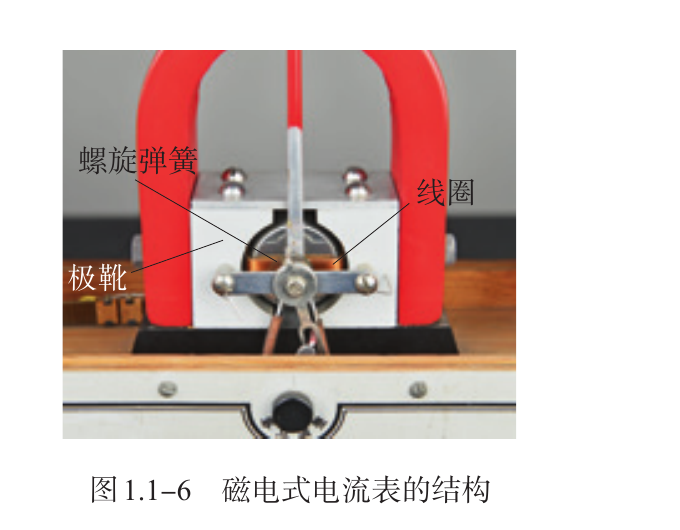
\includegraphics[width=0.40\textwidth]{figures/textbook_1-1-6.png}
\end{figure}

\begin{itemize}
    \item \textbf{基本组成：}磁体、磁极间的线圈、转轴、指针和螺旋弹簧。
    \item \textbf{转动原因：}电流通过线圈时，线圈两侧导线所受安培力方向相反，形成使线圈转动的力矩。
    \item \textbf{指针偏转：}线圈带动指针转动，同时螺旋弹簧发生形变并产生反向作用；达到平衡时，指针停在某一偏角。
    \item \textbf{读数原理：}电流越大，安培力及平衡偏角通常越大，因此可由指针偏转反映电流大小。电流方向改变时，偏转方向也改变。
    \item \textbf{径向磁场：}极靴与铁质圆柱使磁场沿半径方向分布。线圈转动时，线圈平面与磁感线保持平行，线圈两侧所受安培力形成稳定的转动力矩。
    \item \textbf{特点：}磁电式电流表灵敏度高，能测量较弱的电流；其线圈导线较细，允许通过的电流较弱。
\end{itemize}

\begin{figure}[htbp]
    \centering
    \begin{minipage}{0.42\textwidth}
        \centering
        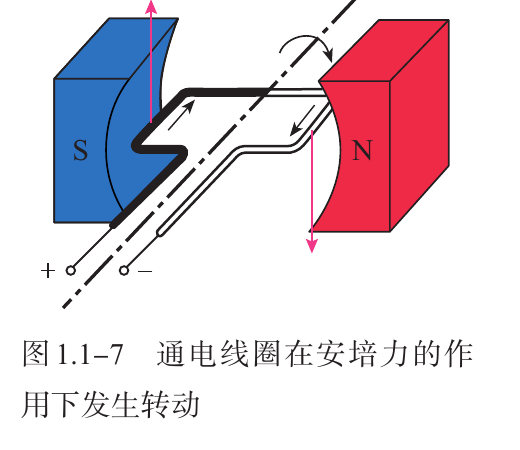
\includegraphics[width=\linewidth]{figures/textbook_1-1-7.png}
    \end{minipage}\hfill
    \begin{minipage}{0.49\textwidth}
        \centering
        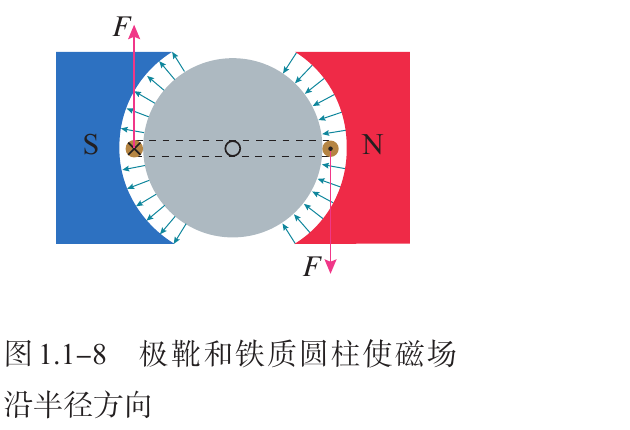
\includegraphics[width=\linewidth]{figures/textbook_1-1-8.png}
    \end{minipage}
\end{figure}

\begin{formal}
    \noindent\textbf{工作过程}\quad 电流通过线圈 \(\longrightarrow\) 线圈受安培力而转动 \(\longrightarrow\) 指针偏转、弹簧形变 \(\longrightarrow\) 达到平衡后由偏角反映电流。
\end{formal}


\section{洛伦兹力}

\subsection{洛伦兹力的产生}
运动电荷在磁场中受到的力称为洛伦兹力。通电导线中的定向运动电荷受到的洛伦兹力的宏观表现，就是安培力。
\begin{itemize}
    \item 洛伦兹力的研究对象是运动电荷。
    \item 静止电荷在磁场中不受洛伦兹力。
\end{itemize}


\subsection{洛伦兹力的方向：左手定则}
\begin{enumerate}
    \item 伸开左手，使拇指与其余四指垂直，并与手掌处于同一平面。
    \item 让磁感线垂直进入掌心。
    \item 对正电荷，使四指指向电荷运动方向，拇指所指就是洛伦兹力方向。
\end{enumerate}
\begin{itemize}
    \item 对负电荷，四指应指向其运动方向的反方向；也可先按正电荷运动方向判断，再将结果反向。
    \item 洛伦兹力方向始终垂直于速度方向和磁感应强度方向。
\end{itemize}


\subsection{洛伦兹力的大小}
设带电粒子的电荷量大小为 \(|q|\)，速度大小为 \(v\)，磁感应强度大小为 \(B\)，速度方向与磁场方向夹角为 \(\theta\)，则
\[
    F=|q|vB\sin\theta.
\]
\begin{itemize}
    \item 当 \(v\perp B\) 时，\(F=|q|vB\)。
    \item 当 \(v\parallel B\) 或 \(v=0\) 时，\(F=0\)。
    \item 电荷正负影响洛伦兹力方向，不影响大小公式中的电荷量大小 \(|q|\)。
\end{itemize}


\subsection{洛伦兹力的作用特点}
\begin{itemize}
    \item 洛伦兹力始终与粒子速度垂直，因此它不对粒子做功。
    \item 若粒子只受洛伦兹力，磁场只改变速度方向，不改变速度大小。
    \item 分析方向时先辨明电荷正负，再使用左手定则；分析大小时先判断速度与磁场的夹角。
\end{itemize}


\section{磁场模型}
% 三类圆模型均按边界形状整理。

\subsection{平移圆}

\subsubsection{直线边界}

\subsubsection{三角形边界}

\subsubsection{圆形边界}

% 在目录中保持“缩放圆”及其三类边界标题同页。
\addtocontents{toc}{\protect\newpage}

\subsection{缩放圆}

\subsubsection{直线边界}

\subsubsection{三角形边界}

\subsubsection{圆形边界}


\subsection{旋转圆}

\subsubsection{直线边界}

\subsubsection{三角形边界}

\subsubsection{圆形边界}


\section{组合场}

\subsection{组合方式}

\subsubsection{双磁场}

\subsubsection{先电场后磁场}

\subsubsection{先磁场后电场}

\subsection{组合场的应用}

\subsubsection{质谱仪}

\subsubsection{回旋加速器}


\section{叠加场}

\subsection{运动类型}

\subsubsection{匀速直线运动}

\subsubsection{匀速圆周运动}

\subsubsection{复杂曲线运动：配速法}

\subsection{叠加场的应用}

\subsubsection{速度选择器}
\begin{figure}[H]
    \centering
    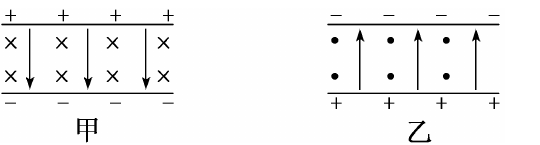
\includegraphics[width=0.58\textwidth]{figures/app_velocity_selector.png}
\end{figure}

\subsubsection{磁流体发电机}
\begin{figure}[H]
    \centering
    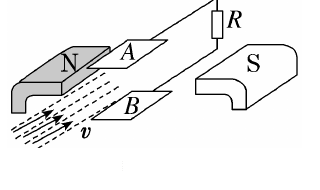
\includegraphics[width=0.42\textwidth]{figures/app_mhd_generator.png}
\end{figure}

\subsubsection{电磁流量计}
\begin{figure}[H]
    \centering
    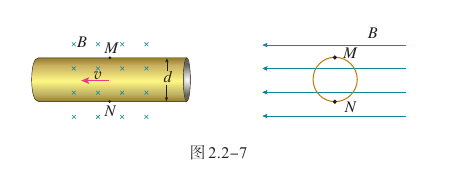
\includegraphics[width=0.58\textwidth]{figures/app_electromagnetic_flowmeter.png}
\end{figure}

\subsubsection{霍尔元件}
\begin{figure}[H]
    \centering
    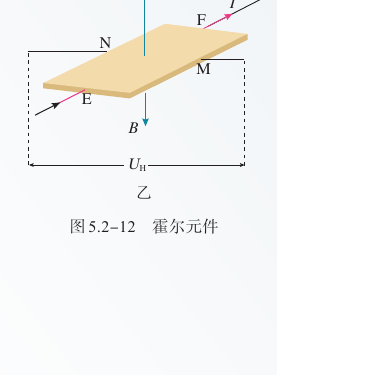
\includegraphics[width=0.35\textwidth]{figures/app_hall_element.png}
\end{figure}


\section{立体空间中的运动}

\subsection{螺线与旋进}

\subsection{立体空间中的偏转}

\end{document}
